\documentclass{report}

\usepackage{textcomp}
\usepackage{graphicx}
\usepackage{minted}
\usepackage{fancyhdr}
\usepackage{subcaption}
\usepackage{multicol}
\usepackage{outlines}
%===================================
\newcommand{\classinfo}{{\bf RHEL 134 \\ Week 1 Lab}\\{\it CIT 218}\\{Chaz Davis}}
\newcommand{\semester}{BCTC \\ Spring 2020}
%===================================
\newcommand{\mysection}[1]{\section*{#1}}
\newcommand{\mysubsection}[2]{\textbf{\romannumeral #1) #2}}
%===================================
\setlength{\headheight}{15.2pt}
\pagestyle{fancy}
\fancyhf{}
\lhead{ \fancyplain{}{Chaz Davis} }
\rhead{ \fancyplain{}{\today} }
\cfoot{ \fancyplain{}{\thepage} }
\renewcommand{\headrulewidth}{0.5pt}
\renewcommand{\footrulewidth}{0pt}

%===================================
\title{\classinfo}
\author{\semester}
\date{\today}

%===================================

\begin{document}

\maketitle

%===================================
\mysection{\textbf{Questions}}

\mysubsection{1}{Use grep to find all the log entries in /var/log/messages
regarding the Hostname service and provide the output}
\\You can see in Fig.~\ref{Ch02}\subref{Ch02Host} 
on Pg.~\pageref{Ch02}, I ran the command 
{\scriptsize{\verb$grep 'Hostname' /var/log/messages$}\normalsize} from the
terminal.

\noindent\mysubsection{2}{Using tail and grep, provide the last 5 entries of
/var/log/messages that start with the month of March}
\\You can see in Fig.~\ref{Ch02}\subref{Ch02Mar} 
on Pg.~\pageref{Ch02}, I ran the command
{\scriptsize{\verb$grep '^Mar' /var/log/messages | tail -n 5$}\normalsize} 
in the terminal to get the last 5 entries for the month of March.

\noindent\mysubsection{3}{Using vim, create a short bash script that pings
8.8.8.8 with 1 ping packet. If the command is successful, print "SUCCESS". If
the command is unsuccessful, print "FAILURE". Send all output from the ping
command to /dev/null. Provide your script and the results of running your
script}
\\You can see in Fig.~\ref{Ch03}\subref{Ch03Vim} 
on Pg.~\pageref{Ch03}, I wrote a simple bash script in vim:
\begin{minted}
[
frame=lines,
framesep=2mm,
baselinestretch=1.2,
fontsize=\footnotesize,
linenos
]
{bash}
#! /usr/bin/bash
ping -c1 8.8.8.8 > /dev/null
if [ $? -eq 0 ]
  then
    echo "SUCCESS"
    exit 0
  else
    echo "FAILURE"
fi
\end{minted}

Where ping -c1 means send the ping command only once, then the ipaddress, The
output of which will be sent to /dev/null.
Then, using an if/else statement I'm using [ \$? -eq 0 ] to get the exit status
of the most recently run command, 0 being true, anything else being no or an
error. and if the exit status was 0, then print "SUCCESS", but if its not true
(else) print "FAILURE" to the comandline. I also realized when I was going to
run the script I forgot to make it executable and so ran
{\scriptsize{\verb$sudo chmod +x ping.sh$}\normalsize}. Then, I was able to run
{\scriptsize{\verb$./ping.sh$}\normalsize}. You can see in
Fig.~\ref{Ch03}\subref{Ch03Ping} 
on Pg.~\pageref{Ch03}, that we got "FAILURE".


\begin{figure}[!hbt]\centering
\subfloat[Grepping Hostname]{\label{Ch02Host}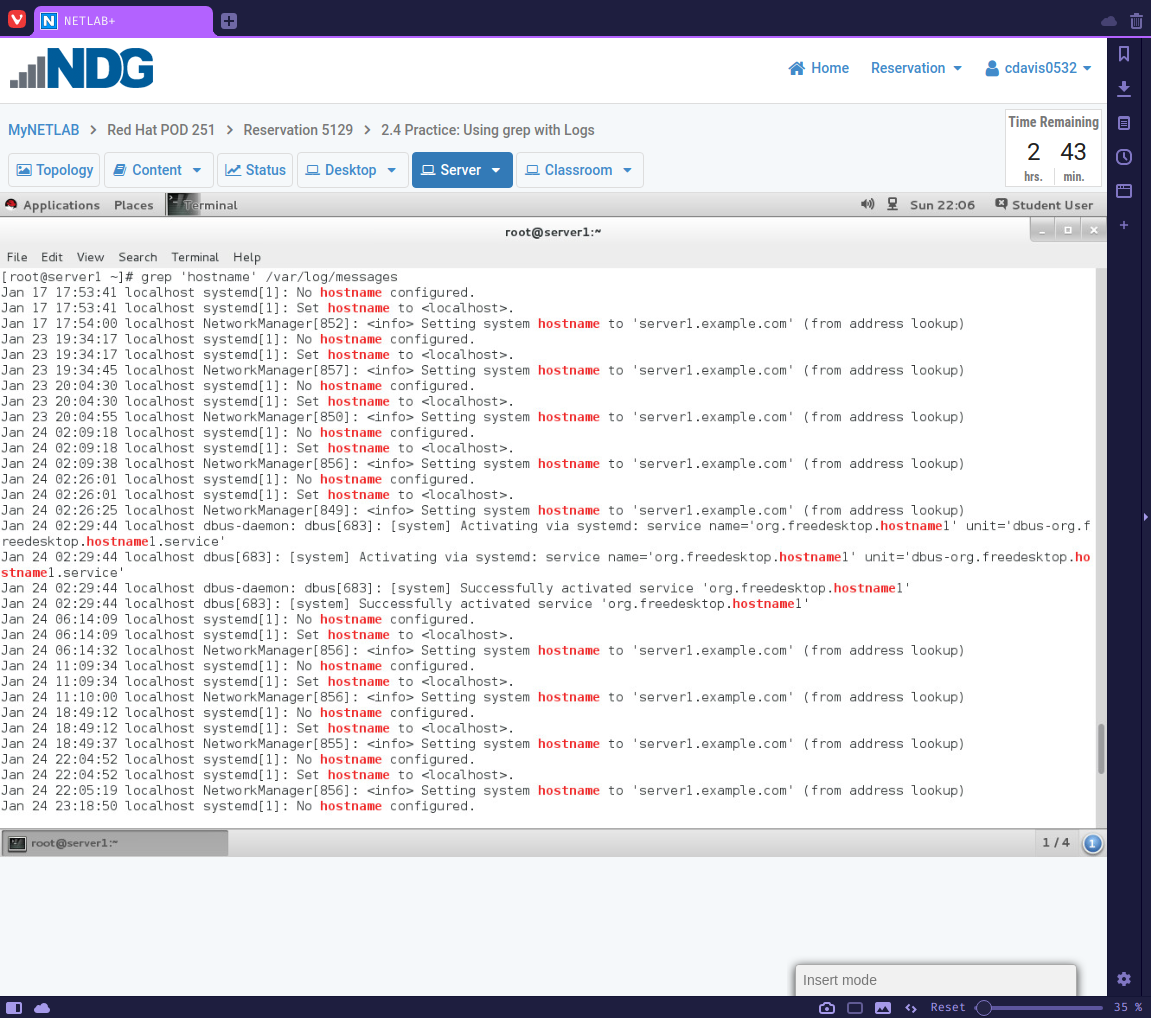
\includegraphics[width=.95\linewidth]{Figures/2020-03-08-220621_1151x1018_scrot.png}}\par
\subfloat[Grepping the last five entries for March]{\label{Ch02Mar}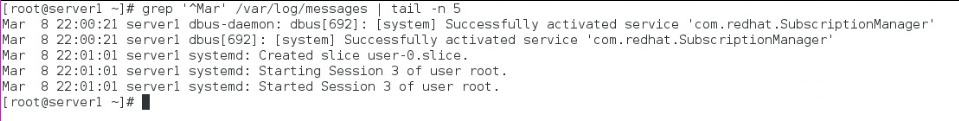
\includegraphics[width=.95\linewidth]{Figures/2020-03-08-220831_959x121_scrot.png}}\par
\caption{Chapter 02 Screenshots}
\label{Ch02}
\end{figure}

\begin{figure}[!hbt]\centering
\subfloat[Writing my bash script insidevim]{\label{Ch03Vim}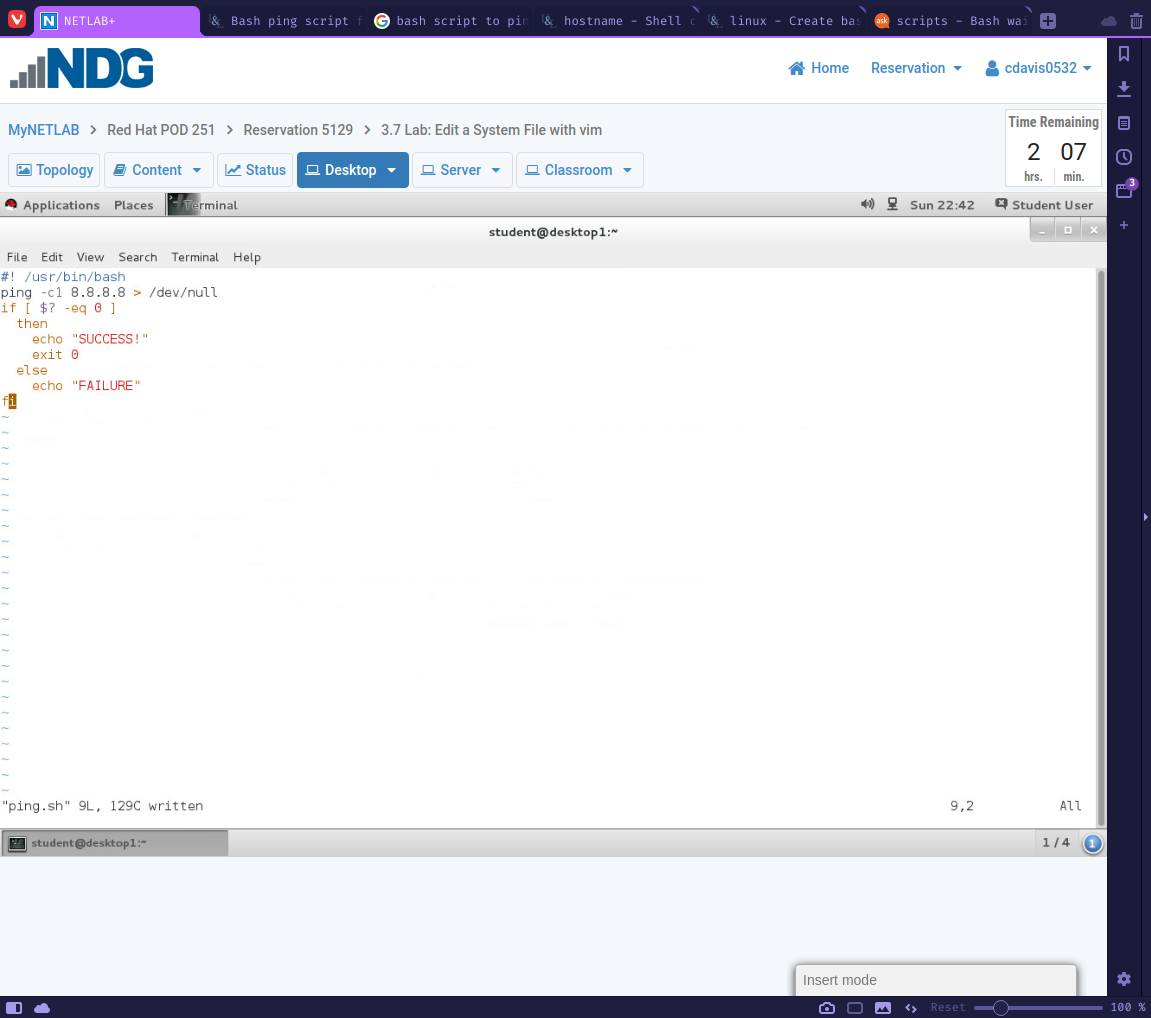
\includegraphics[width=.95\linewidth]{Figures/2020-03-08-224208_1151x1018_scrot.png}}\par
\subfloat[Running my Bash script from thecommandline]{\label{Ch03Ping}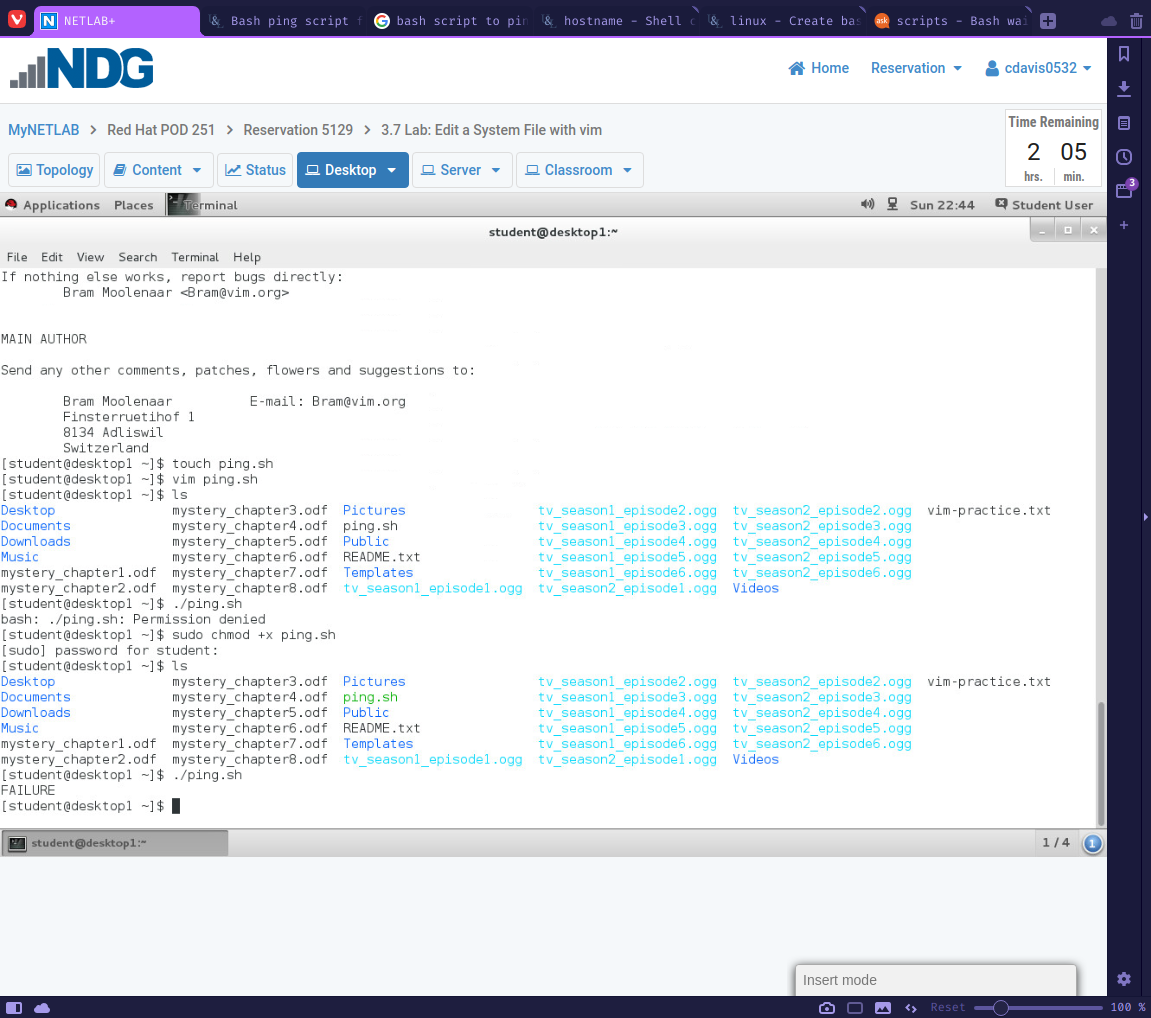
\includegraphics[width=.95\linewidth]{Figures/2020-03-08-224401_1151x1018_scrot.png}}\par
\caption{Chapter 03 Screenshots}
\label{Ch03}
\end{figure}

%===================================

\end{document}
